\begin{pastexam}[label={px:ncku-109-ee-ds-03}]{成大電機所 109 學年度 第 3 題}
（問答；15 分）

The following array represents a complete binary tree. Adjust it to be a max heap by
\textbf{showing each step}. \quad (15 points)
\begin{center}
\begin{tabular}{|*{10}{c|}}
\hline
10 & 9 & 20 & 6 & 15 & 48 & 14 & 8 & 90 & 17 \\ \hline
\end{tabular}
\end{center}
\end{pastexam}

\begin{pastsoln}
最後的最大堆積是 $[90, 17, 48, 9, 15, 20, 14, 8, 6, 10]$。

用由下往上的建堆積（資結書第~8.2~節、虛擬碼~8.3）：陣列從 $1$ 開始編號，$n = 10$，從最後一個
內部節點 $\lfloor n/2 \rfloor = 5$ 往前到 $1$，每個節點往下調整（和較大的子節點比，比它小就交換，
一路往下直到不必換）。 位置 $i$ 的子節點是 $2i$、$2i + 1$。 原來的樹：
\begin{center}
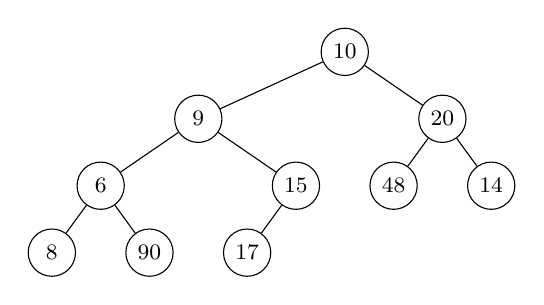
\begin{tikzpicture}[baseline=(current bounding box.center),every node/.style={circle,draw,minimum size=6mm,inner sep=0pt,font=\footnotesize}]
\node[] (n8) at (0.00,-2.55) {8};
\node[] (n6) at (0.62,-1.70) {6};
\node[] (n90) at (1.24,-2.55) {90};
\node[] (n9) at (1.86,-0.85) {9};
\node[] (n17) at (2.48,-2.55) {17};
\node[] (n15) at (3.10,-1.70) {15};
\node[] (n10) at (3.72,0.00) {10};
\node[] (n48) at (4.34,-1.70) {48};
\node[] (n20) at (4.96,-0.85) {20};
\node[] (n14) at (5.58,-1.70) {14};
\draw (n6) -- (n8);
\draw (n6) -- (n90);
\draw (n15) -- (n17);
\draw (n9) -- (n6);
\draw (n9) -- (n15);
\draw (n20) -- (n48);
\draw (n20) -- (n14);
\draw (n10) -- (n9);
\draw (n10) -- (n20);
\end{tikzpicture}
\end{center}

\begin{center}
\small
\begin{tabular}{clll}
\toprule
調整 & 節點（值） & 交換 & 調整後的陣列 \\
\midrule
開始 & & & $[10, 9, 20, 6, 15, 48, 14, 8, 90, 17]$ \\
1 & 位置 5（15） & $15 \leftrightarrow 17$（位置 10） & $[10, 9, 20, 6, \mathbf{17}, 48, 14, 8, 90, \mathbf{15}]$ \\
2 & 位置 4（6） & $6 \leftrightarrow 90$（位置 9） & $[10, 9, 20, \mathbf{90}, 17, 48, 14, 8, \mathbf{6}, 15]$ \\
3 & 位置 3（20） & $20 \leftrightarrow 48$（位置 6） & $[10, 9, \mathbf{48}, 90, 17, \mathbf{20}, 14, 8, 6, 15]$ \\
4 & 位置 2（9） & $9 \leftrightarrow 90$（位置 4） & $[10, \mathbf{90}, 48, \mathbf{9}, 17, 20, 14, 8, 6, 15]$ \\
5 & 位置 1（10） & $10 \leftrightarrow 90$（位置 2） & $[\mathbf{90}, \mathbf{10}, 48, 9, 17, 20, 14, 8, 6, 15]$ \\
  &              & $10 \leftrightarrow 17$（位置 5） & $[90, \mathbf{17}, 48, 9, \mathbf{10}, 20, 14, 8, 6, 15]$ \\
  &              & $10 \leftrightarrow 15$（位置 10） & $[90, 17, 48, 9, \mathbf{15}, 20, 14, 8, 6, \mathbf{10}]$ \\
\bottomrule
\end{tabular}
\end{center}
說明：
\begin{itemize}
\item 位置 5 的 $15$ 只有一個子節點 $17$，$15 < 17$，交換。
\item 位置 4 的 $6$，子節點 $8$、$90$，較大的是 $90$，交換；$6$ 到了位置 9，是樹葉，停。
\item 位置 3 的 $20$，子節點 $48$、$14$，和 $48$ 交換；到位置 6，是樹葉，停。
\item 位置 2 的 $9$，子節點 $90$、$17$，和 $90$ 交換；到位置 4，子節點 $8$、$6$ 都比 $9$ 小，停。
\item 位置 1 的 $10$，子節點 $90$、$48$，和 $90$ 交換；到位置 2，子節點 $9$、$17$，和 $17$ 交換；
到位置 5，子節點只有 $15$，和 $15$ 交換；到位置 10，是樹葉，停。
\end{itemize}
最後的最大堆積：
\begin{center}
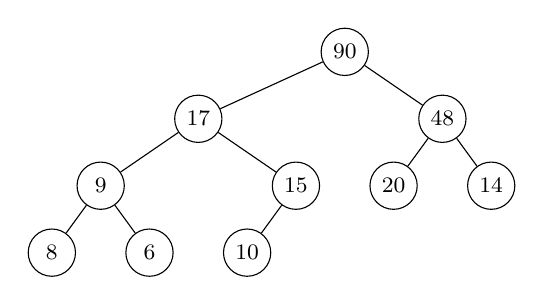
\begin{tikzpicture}[baseline=(current bounding box.center),every node/.style={circle,draw,minimum size=6mm,inner sep=0pt,font=\footnotesize}]
\node[] (n8) at (0.00,-2.55) {8};
\node[] (n9) at (0.62,-1.70) {9};
\node[] (n6) at (1.24,-2.55) {6};
\node[] (n17) at (1.86,-0.85) {17};
\node[] (n10) at (2.48,-2.55) {10};
\node[] (n15) at (3.10,-1.70) {15};
\node[] (n90) at (3.72,0.00) {90};
\node[] (n20) at (4.34,-1.70) {20};
\node[] (n48) at (4.96,-0.85) {48};
\node[] (n14) at (5.58,-1.70) {14};
\draw (n9) -- (n8);
\draw (n9) -- (n6);
\draw (n15) -- (n10);
\draw (n17) -- (n9);
\draw (n17) -- (n15);
\draw (n48) -- (n20);
\draw (n48) -- (n14);
\draw (n90) -- (n17);
\draw (n90) -- (n48);
\end{tikzpicture}
\end{center}
檢查：每個父節點都不小於子節點（$90 \ge 17, 48$；$17 \ge 9, 15$；$48 \ge 20, 14$；$9 \ge 8, 6$；
$15 \ge 10$）。 由下往上建堆積總共 $O(n)$（資結書定理~8.1）。

若改成「從空堆積開始，依序把這 $10$ 個數插入」，會得到不同的堆積（$[90, 48, 20, 15, 17,\allowbreak
10, 14, 6, 8, 9]$）；題目說的是把這個陣列\textbf{調整}成堆積，用上面由下往上的做法。
\end{pastsoln}
